% --- chapter
\newcommand{\chapter}[2][]{
	\newcommand{\chapname}{#2}
	\begin{flushleft}
		\begin{minipage}[t]{\linewidth}
			
\includegraphics[height=1cm]{hdht-logo.png}
			\hspace{0pt}	
			\sffamily\bfseries\large Bài  22. Sóng điện từ
			\begin{flushleft}
				\huge\bfseries #1
			\end{flushleft}
		\end{minipage}
	\end{flushleft}
	\vspace{1cm}
	\normalfont\normalsize
}
%-----------------------------------------------------
\chapter[Sóng điện từ và truyền sóng điện từ]{Sóng điện từ và truyền sóng điện từ}

\subsection{Định nghĩa}
Sóng điện từ là điện từ trường lan truyền trong không gian.
\subsection {Đặc điểm}
\begin{itemize}
	\item Sóng điện từ là sóng ngang, lan truyền được trong chân không và trong các môi trường vật chất.
	\item Tốc độ truyền sóng điện từ phụ thuộc vào môi trường truyền sóng; trong chân không, không khí là $c=3.10^8\ \text{m/s}$, trong các môi trường khác, tốc độ nhỏ hơn.
	\item Vectơ cường độ điện trường $\vec{E}$ và vectơ cảm ứng từ $\vec {B}$ luôn luôn vuông góc với nhau và vuông góc với phương truyền sóng. Ba vectơ $\vec{E}, \vec{B}$ và $\vec{v}$ tại mọi điểm tạo với nhau thành một tam diện thuận.
	\begin{center}
		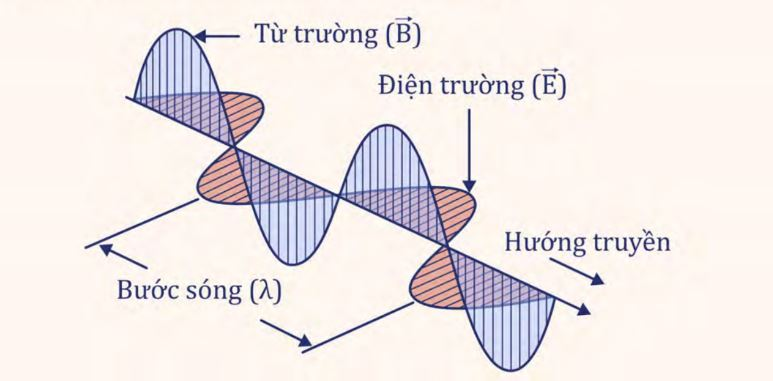
\includegraphics[scale=0.7]{../figs/4-3-1.JPG}
	\end{center}
	\item Dao động của điện trường và của từ trường tại một điểm luôn luôn cùng pha với nhau.
	\item Sóng điện từ tuân theo định luật truyền thẳng, phản xạ, khúc xạ như ánh sáng.
	\item Sóng điện từ mang năng lượng.
	\subsection {Bảng sóng vô tuyến và ứng dụng}
	\begin{tabular}{|m{2cm}|m{2.5cm}|m{13em}|m{8em}|}
		\hline
		\thead{Loại sóng} & \thead{Bước sóng}  & \thead{Đặc điểm}  & \thead{Ứng dụng}  \\
		\hline
		\nfhead{Sóng dài}	& \nfhead{$\geq 1000\ \text{m}$} & Có năng lượng thấp.\newline Bị các vật trên mặt đất hấp thụ mạnh nhưng nước lại hấp thụ ít. & Dùng trong thông tin liên lạc dưới nước. \\
		\hline
		Sóng trung	&$100-1000\ \text{m}$  & Ban ngày bị tầng điện li hấp thụ mạnh nên không truyền đi xa được. \newline Ban đêm bị tầng điện li phản xạ nên truyền đi xa được.  & Dùng trong thông tin liên lạc vào ban đêm. \\
		\hline
		Sóng ngắn	& \nfhead{$10-100\ \text{m}$}  & Có năng lượng lớn. \newline Bị phản xạ nhiều lần giữa tầng điện li và mặt đất.  & Dùng trong thông tin liên lạc trên mặt đất.  \\
		\hline
		\nfhead{Sóng\\ cực ngắn}	&\nfhead{$1-10\ \text{m}$}  &Có năng lượng rất lớn. Không bị tầng điện li hấp thụ hay phản xạ.\newline Xuyên qua tầng điện li vào vũ trụ.  & Dùng trong thông tin vũ trụ. \\
		\hline
	\end{tabular}
\end{itemize}
